\chapter{Deep Reinforcement Learning for non-Markovian goals}

\section{Reinforcement Learning}

% Motivation
In this section we will briefly review the most important aspects of classic
\emph{Reinforcement Learning} (RL). These concepts are relevant because they
are also found in Deep Reinforcement Learning (Deep RL), which is a central
component of the agent we will design. Excellent references for these topics
are \cite{bib:rl-book}, \cite{bib:probabilistic-rl}, and
\cite{bib:ml-book-murphy} for graphical models.

% Agent-env interface
In AI, we commonly isolate two entities, the agent and the environment, which
continuously interact. At each instant, the agent receives observations from
the environment and it executes actions in response. In RL specifically, the
agent observes the current state of the environment and a numerical reward.
The environment produces high rewards in response to desirable events. The
agent's goal is to maximize the rewards received. The basic setup is
illustrated in Figure~\ref{fig:rl}.

\begin{figure}
	\centering
	\begin{tikzpicture}
		\node [block] (agent) {Agent};
		\node [block, below=of agent] (env) {Environment};
		\draw [flow] ([yshift=2mm]env.west) -- ++(-1.2,0) |-
			([yshift=-2mm]agent.west) node [pos=0.3,right] {reward\\$r$};
		\draw [flow] ([yshift=-2mm]env.west) -- ++(-1.5,0) |-
			([yshift=2mm]agent.west) node [pos=0.3,left] {state\\$s$};
		\draw [flow] (agent.east) -| node [pos=0.7,right] {action\\a}
		($(env.east)+(1.2,0)$) -- (env.east);
	\end{tikzpicture}
	\caption{How agent and environment interact in RL.}
	\label{fig:rl}
\end{figure}

% MDP
Most RL algorithms assume that the environment dynamics can be modelled with a
\emph{Markov Decision Process} (MDP). They do so, because under the
independence assumptions taken by MDP, it's possible to efficiently find the
optimal agent's policy. A Markov Decision Process is a tuple $\langle \stateS,
A, T, R, \discount \rangle$, where: $\stateS$ is the set of states of the
environment; $A$ is the action space; $T: \stateS \times A \times \stateS \to
\R$ is the transition function, which, for ${T(s_{t}, a_{t}, s_{t+1})}$,
returns the probability $p(s_{t+1} \given s_{t}, a_{t})$ of the transition
${s_{t} \xrightarrow{a_{t}} s_{t+1}}$; $R: \stateS \times A \times \stateS \to
\R$ is the reward function; and $\discount \in [0, 1]$ is called ``discount
factor''\footnote{In this chapter, a variable with a subscript refers to the
value of the variable at the discrete time indicated.}.

% Markov assumptions
In a RL problem, the functions $T$ and $R$ are unknown. The agent can only
learn them by observing the samples it receives from the environment.
However, by assuming that they can be modelled with functions ${\stateS \times
A \times \stateS \to \R}$, we introduce some Markov assumptions. In
particular, we assume that the next state of the environment is conditionally
independent on the whole history, given the previous state and action:
$s_{t+1} \perp s_{0}, \dots, s_{t-1} \given s_{t}, a_{t}$. Similarly, the
reward only depends on the last transition of the environment.  Although it's
not required by the model, it is common that rewards are computed just from
desirable configurations of the environment~$s_{t}$, not from specific
transitions $(s_{t}, a_{t}, s_{t+1})$. All of these assumptions are summarized
in the Directed Graphical Model (DGM) of Figure~\ref{fig:mdp}. In a DGM,
directed edges indicate direct conditional probabilities, while missing arcs
indicate conditionally independent variables.  In Figure~\ref{fig:mdp}, the
lack of any arrow between $s_{t-1}$ and $s_{t+1}$ means that future states,
hence the rewards, do not depend on the past history, given the current
state~$s_t$.  This is the essence of a Markov assumption.

\begin{figure}
	\centering
	\begin{tikzpicture}
		\matrix [
			column sep={1cm,between origins}, row sep={1cm,between origins},
		] {
			\&
			\node (am1) [node, label=above:$a_{t-1}$] {};
			\& \&
			\node (a) [node, label=above:$a_{t}$] {}; \& \\
			\node (stm1) [node, label=above:$s_{t-1}$] {};
			\& \&
			\node (st) [node, label=above:$s_{t}$] {}; \& \&
			\node (st1) [node, label=above:$s_{t+1}$] {}; \\
			\& \&
			\node (r) [node, label=below:$r_{t}$] {}; \& \&
			\node (r1) [node, label=below:$r_{t+1}$] {}; \\
		};
		\draw (st1) edge [<-] (st) edge [<-] (a);
		\draw [->, dotted] (st) -- (a);
		\draw [->] (st) -- (r);
		\draw [->] (st1) -- (r1);
		\draw (st) edge [<-] (stm1) edge [<-] (am1);
		\draw [->, dotted] (stm1) -- (am1);

		\draw [dashed, gray] (st1) -- +(0.8,0);
		\draw [dashed, gray] (stm1) -- +(-0.8,0);
	\end{tikzpicture}
	\caption{The directed graphical model of a MDP.}
	\label{fig:mdp}
\end{figure}

\begin{example}
	\label{ex:board-games}
	Tic-Tac-Toe, Chess and many other board games can be modelled with an MDP.
	Even games with dice, such as Backgammon. To do so, we define as state
	space~$\stateS$ the set of configurations of the board; as reward
	function~$R(s)$ = 1, if the configuration $s$ is a win, $-1$ for a lose, 0
	otherwise. Even though most games are deterministic, the presence of an
	opponent makes the transition function~$T$ of the MDP nondeterministic.
	What these games have in common, is that the player gets to see the complete
	state of the game, which is the current configuration of the board. Future
	states of the game and rewards only depend on the current situation, not on
	the whole play. In Chess, for example, we can determine whether a
	configuration is a win or loss just by looking for a checkmate, there is no
	need to ask the players how the game has carried out.

	Proving that Markovian $T$ and $R$ exist is easy for board games, because
	the rules of the game define them. As we will see in
	Section~\ref{sec:non-markov}, when $T$ is unknown, as always happens in the
	real-world, it's much more difficult to prove that we're in fact facing a
	MDP.
\end{example}

The \emph{policy} is the criterion the agent uses to select the actions to
perform. If the environment dynamics can be modelled with a MDP, the
optimal action at time~$t$ only depends on~$s_{t}$. So, there must exist
an optimal policy as $\policy^*: \stateS \to A$. Due to common estimation
errors, it is always better to prefer nondeterministic policies, which return
a probability distribution over the actions. The action at time $t$ will be
sampled according to $a_t \sim \policy(s_t)$. This dependency is represented
by the dotted arrows of Figure~\ref{fig:mdp}.

We will now introduce few basic quantities of RL that serve to define what it
means for an action or a policy to be optimal. The \emph{discounted
return}~$G$ is the combination of all rewards collected:
\begin{equation}
	G \coloneqq r_{0} + \discount\, r_1 + \discount^2 r_2 + \dots =
	\sum_{t=0}^{T} \discount^{t} r_{t}
	\label{eq:return}
\end{equation}
The discount factor, $0 \le \discount \le 1$, decides the relative importance
of immediate and future rewards. Usually, this factor is strictly less than 1
because this stimulates the agent to achieve rewards as soon as possible.
It also produces a finite discounted reward, even for an infinite run $T \to
\infty$.  Since our environments are video games, each play is an episode and
the total number of steps in each episode is finite.

It is now clear, that the optimal policy should always maximize the expected
discounted return. The \emph{value function} of a policy $\policy$ computes
this quantity for each state $s$:
\begin{equation}
	v_{\policy}(s) \coloneqq \E_{\policy}[G \given s_0 = s]
\end{equation}
which computes the expected value of $G$, when the agent starts from state $s$
and it follows the policy~$\policy$. The notation $\E_{\policy}$ indicates
that the estimation assumes that the actions are sampled according
to~$\policy$. Finally, we can define the \emph{optimal policy} $\policy^*$ as
the one maximizing the value function at all states:
\begin{equation}
	\policy^*: \quad v_{\policy^*}(s) \ge v_{\policy}(s) \qquad \forall s \in
	\stateS, \quad \text{for all $\policy$}
\end{equation}
The typical Reinforcement Learning problem is to find the optimal policy for
an MDP with unknown $T$ and~$R$.

The \emph{action-value function} of a policy $\policy$ is a similar measure to
the value function:
\begin{equation}
	q_{\policy}(s, a) \coloneqq \E_{\policy}[G \given s_0 = s, a_0 = a]
\end{equation}
that forces the first action to be~$a$. Since the agent only observes outcomes
of single actions, this is usually a much more convenient form for updating
the estimate of the expected discounted return. Also, the optimal policy can
be simply expressed as:
\begin{equation}
	\policy^*(s) = \argmax_{a \in A} q_{\policy^*}(s, a)
\end{equation}
So, instead of learning the optimal policy directly, we can learn the optimal
state-value function,~$q_{\policy^*}$ (also denoted with $q^*$). Fortunately,
we don't need $\policy^*$ to valuate $q^*$ because, assuming optimality, we
know it satisfies the Bellman optimality equation:
\begin{align}
	q^*(s, a) &= \E\, \bigl[ r_{t+1} + \discount \max_{a'} q^*(s_{t+1}, a')
	\given s_t = s, a_t = a \bigr] \\
	&= \sum_{s', r'} p(s', r' \given s, a) \,
	\bigl( r' + \discount \max_{a'} q^*(s', a') \bigr)
\end{align}
for any~$t$.

Many learning algorithms exist for estimating $q^*$. Briefly, on-policy
algorithms, estimate $q_\policy$ of the policy currently in use $\policy \to
\policy^*$; off-policy algorithms, instead, act according to any exploration
policy $\policy'$ and directly estimate $q^*$. Two famous algorithms in these
classes are SARSA and Q-learning, respectively. The one used in this thesis is
derived from the latter.


\section{Deep Reinforcement Learning}

Classic RL algorithms, such as SARSA and Q-learning, are tabular methods
because they store and update the estimate for each pair $(s, a)$
independently. Unfortunately, this requires discrete and small states and
actions spaces. To overcome this very limiting assumption, we need
parametrized value functions and policies.  \emph{Deep Reinforcement Learning}
(Deep RL) is a recent field of RL in which Neural Networks (NN) are used as
powerful function approximators for policies or value functions.

The main advantage of NN, and parametric models in general, is that they can
be trained in high-dimensional and continuous input spaces. In fact, a good
fit does not require a complete exploration of the input space, which may be
unfeasible or impossible. Instead, they are trained with some form of
Stochastic Gradient Descent (SGD) on the set of parameters from input-output
samples. Then, the model will be able to generalize to inputs that have been
never observed.

Deep RL algorithms allow very little guarantees about convergence and
optimality.  Even if the input space would be explored completely, due to
parametrization, updates for recent samples also affect the regions previously
visited. In fact, any Deep RL algorithm introduces some techniques in order to
generate a stable training.

The Deep Q-Network (DQN)~\cite{bib:atari-deeprl} is an important algorithm
because it successfully combined previous techniques for a stable training,
and an interesting model based on deep NN for the state-value function.
The outcome is very satisfactory: the same neto
This resulted in an 
They demonstrated that the same network can be trained in different games and
achieve These promising
results sparked a lively interest in Deep RL.



% TODO We'll only deal with discrete action spaces, where the policy
% is a categorical distribution (a vector of probabilities).



\section{Temporal logics and Linear Dynamic Logic}

\subsection{Temporal logics on finite traces}

% Intro to temporal logics
Temporal logics are a class of formal languages, more precisely modal logics,
that allow to talk about time~\cite{bib:temporal-logics-stanford}. Among all
formalisms, we care about logics that assume a linear time, as opposed to
branching, and a discrete sequence of instants, instead of continuous time.
In computer science, the most famous logic in this group is the Pnueli's
Linear Temporal Logic (LTL)~\cite{bib:pnueli-ltl}.

% Structures
The assumptions about the nature of time directly reflect to the type of
structures these logics are interpreted on: their models are $\modelsym =
\langle T, \prec, V \rangle$, where the set $T$ is a discrete set of time
instants, such as $\N$, and $\prec$ is a complete ordering relation on $T$,
like~$<$. If a logic defines a set $\fluents$ of atomic propositions, the
evaluation function $V: T \times \fluents \to \{\true, \false\}$, for each
instant of time, assigns a truth value to each fluent. An equivalent and
compact way of defining such structures is with \emph{traces}. A trace
$\trace$ is a sequence of propositional interpretations $2^\fluents$ of the 
fluents~$\fluents$. Each element of the trace, $\trace(i)$, is the set of true
symbols at time~$i$. $\trace(i, j)$ represents the trace between instants $i$
and~$j$.
% TODO: evaluation or valuation?

% Structures in LTL
LTL is a logic that only allows to talk about the future. The semantic of its
temporal operators, neXt~$\next$, Until~$\until$, and of those derived,
eventually~$\eventually$, always~$\always$, can only access future instants on
the sequence. Interpretations for this logic are infinite traces with a first
instant, which are equivalent to valuations on the temporal frame $\langle \N,
< \rangle$.

% Finite traces
As it has been pointed out~\cite{bib:ltlf-ldlf}, most practical uses of LTL
interpret the formulae on \emph{finite} traces, not infinite. The pure
existence of a last instant of time has strong consequences on the meaning of
the operators, because they need to handle such instant differently. The
Always operator~$\always$, translates to ``until the last instant'', quite
naturally. However, writing $\always\eventually \formula$ does not require
that $\formula$ becomes true an infinite number of times, that is the
``response'' property; instead, it is satisfied exactly by those traces in
which $\formula$ is true at $\const{Last}$ ($\const{Last}$ is an abbreviation
for $\lnot \next \true$ and it evaluates to true at last instant only).
Furthermore $\always\eventually \formula$ and $\eventually\always \formula$
are both equivalent to $\eventually (\const{Last} \land \formula)$, something
that doesn't happen in standard LTL. From last example, it should be clear
that the expressive power of the language has changed and LTL interpreted over
finite traces should be regarded as a different logic, that we denote with
\ltl{}. More precisely, over infinite linearly-ordered interpretations, LTL
has the same expressive power of Monadic Second Order Logic (MSO), while
\ltl{} is equivalent to First-Order Logic (FOL) and star-free regular
expressions, which are strictly less expressive.

% Every finite is fine
In the next section, we will define a temporal logic, called \ldl{}, that is
purposefully devised for finite traces. This is the formalism that we use in
the implemented construction for RL agents. However, many plans and behaviours
to be rewarded can be also expressed with~\ltl{}. So, for this construction,
any temporal logic over finite traces which can be translated to equivalent
finite-state automata can be used as an alternative to~\ldl{}; even temporal
logics of the past~\cite{bib:nmrdp-logic-first}.


\subsection{Linear Dynamic Logic}

In this section, we will define Linear Dynamic Logic of finite traces
(\ldl{})~\cite{bib:ltlf-ldlf}. Its syntax combines regular expressions and
propositional logic, just like Propositional Dynamic Logic (PDL)
does~\cite{bib:pdl}\cite{bib:pdl-stanford}. So, we will review regular
expressions first.


\subsubsection{Regular Temporal Specifications}

Regular languages are the class of languages exactly recognized by finite
state automata and regular expressions~\cite{bib:languages-book}. So, we will
use regular expressions as a compact formalism to specify them. Regular
expressions are usually said to accept strings. Traces are in fact strings,
whose symbols $s \in 2^{\fluents}$ are propositional interpretations of the
fluents~$\fluents$. Such regular expressions would be:
\begin{equation}
	\resym ::= \emptyset \mid s \mid
	\resym_1 + \resym_2 \mid \resym_1 ; \resym_2 \mid \resym^*
	\label{eq:re-no}
\end{equation}
where $\emptyset$ denotes the empty language, $s \in 2^\fluents$ is a symbol,
$+$ is the disjunction of two constraints, $;$ separates concatenated
expressions, and $\resym^*$ requires an arbitrary repetition on $\resym$.
Parentheses can be used to group expressions with any precedence.

We call the regular expressions of equation~\eqref{eq:re-no} Regular Temporal
Specifications \re{}, because they are interpreted on finite linear temporal
structures. However, writing specifications in terms of single interpretations
is very cumbersome. So, we substitute the symbols $s \in 2^\fluents$ with
formulae of Propositional Logic. A propositional formula $\propformula$
represents all interpretations that satisfy it: $\text{Sat}(\propformula) = \{s
\in 2^\fluents \mid s \models \propformula\}$.

The new definition for the syntax of Regular Temporal Specifications \re{}:
\begin{equation}
	\resym ::= \propformula \mid
	\resym_1 + \resym_2 \mid \resym_1 ; \resym_2 \mid \resym^*
	\label{eq:re}
\end{equation}
where $\propformula$ is a propositional formula on the set of atomic
symbols~$\fluents$. The language generated by a \re{}~$\resym$, denoted
$\langsym(\resym)$, is the set of traces that match the temporal
specification. The only difference with regular expressions' standard
semantics is that a symbol $s \in 2^\fluents$ matches a propositional formula
$\propformula$ if and only if $s \in \text{Sat}(\propformula)$. A trace that
match the regular expression $\trace \in \langsym(\resym)$ is said to be
generated or accepted by the specification~$\resym$.

\begin{example}
	As an example, let's define a \re{} expression $\resym \coloneqq \true;
	(\lnot B)^*; (A \land B)$ and the following traces:
	\begin{align*}
		\trace_1 &\coloneqq \langle \set{}; \set{A}; \set{A}; \set{A,B} \rangle \\
		\trace_2 &\coloneqq \langle \set{B}; \set{A,B} \rangle \\
		\trace_3 &\coloneqq \langle \set{A, B}; \set{B}; \set{B} \rangle \\
	\end{align*}
	The first two traces are accepted by the expression, $\trace_1, \trace_2 \in
	\langsym(\resym)$, but the third is not, $\trace_3 \not\in
	\langsym(\resym)$. Of course, the symbols $A$ and $B$ could represent any
	meaningful property of the environment to be ensured.
\end{example}


\subsubsection{Linear Dynamic Logic}

Linear Dynamic Logic is a temporal logic for finite traces that was first
defined in~\cite{bib:ltlf-ldlf}. The definition we see here, also adopted by
the implementation we'll use, is a small variant that can also be interpreted
over the empty trace, $\trace_\epsilon = \langle \rangle$, unlike most logics
that assume a non-empty temporal domain~$T$.

\begin{definition}
	A \ldl{} formula $\formula$ is built as follows:
	\begin{equation}
	\begin{aligned}
		\formula \quad &::= \quad \ltt \mid \lnot \formula \mid \formula_1 \land
			\formula_2 \mid \langle \resym \rangle \formula \\
		\resym \quad &::= \quad \propformula \mid \formula? \mid \resym_1 +
			\resym_2 \mid \resym_1; \resym_2 \mid \resym^* \\
	\end{aligned}
	\label{eq:ldl-syntax}
	\end{equation}
	where $\ltt$ is a constant that stands for logical true and $\propformula$
	is a propositional formula over a set of symbols~$\fluents$.
\end{definition}

The syntax just defined is really similar to PDL~\cite{bib:pdl}, a well known
and successful formalism in Computer Science for describing states and events
of programs. However, \ldl{} formulae are interpreted over finite traces
instead of Labelled Transition Systems.

Before moving to the semantics, we can intuitively understand the meaning of
the constructs. The second line of definition~\eqref{eq:ldl-syntax} is a
Regular Temporal Specification \re{}, with the addition of the test
operator~$?$, typical of PDL. In $\langle \resym \rangle \formula$, the \re{}
expression $\resym$ is used as a modal operator to move to future states: it
states that there exists at least one 


\section{Non-Markovian goals}
\label{sec:non-markov}

The goal of a RL agent is to maximize the rewards received.  A goal, or a
task, is said \emph{non-Markovian} if the rewards do not satisfy the Markov
assumption on rewards, i.e:
\begin{equation}
	r_{t+1} \not\perp s_i, a_i, r_i \quad 0 \le i < t \qquad \text{for some $t$}
	\label{eq:markov-rewards}
\end{equation}
% TODO: the above equation should have o_i not s_i, notation?
Of course, this can happen only if the environment cannot be modelled with an
MDP. Excellent algorithms exists for MDPs; instead, non-Markovian goals are
much more difficult to learn.  There are two main causes for non-Markovian
rewards: partial observations and temporally-extended tasks. We'll thoroughly
analyze both scenarios.


\subsection{Partial observations}

Up to this point, we didn't need to distinguish between observations and
states. In fact, we assumed that the agent can directly observe the
environment states and act accordingly (we defined the policy as a function of
the state). Unfortunately, this is often not the case: we only get to see
something that depends on the current state, but it's not. These systems can
be modelled with a \emph{Partially Observable Markov Decision Process}
(POMDP).  POMDPs are a generalization of MDPs for partial observations. From
now on, we will denote with $\stateS$ the environment state space and with
$\obsS$ the observation space. Formally, a discrete-time POMDP is a 7-tuple
${\langle \stateS, A, T, R, \obsS, O, \discount \rangle}$, where $\stateS, A,
T, R$ are defined as usual, $\obsS$ is the observation space, and $O$ is the
observation function ${O: S \to \obsS}$.

The graphical model of a POMDP is shown in Figure~\ref{fig:pomdp}.
\begin{figure}
	\centering
	\begin{tikzpicture}
		\matrix [
			column sep={1.5cm,between origins}, row sep={1cm,between origins},
			hidden node/.style={node, fill=gray},
		] {
			\node (om1) [node, label=above:$o_{t-1}$] {}; \&
			\node (am1) [node, label=above:$a_{t-1}$] {}; \&
			\node (o) [node, label=above:$o_{t}$] {}; \&
			\node (a) [node, label=above:$a_{t}$] {}; \\
			\node (stm1) [hidden node, label=below left:$s_{t-1}$] {};
			\& \&
			\node (st) [hidden node, label=below left:$s_{t}$] {}; \& \&
			\node (st1) [hidden node, label=below left:$s_{t+1}$] {}; \\
			\& \&
			\node (r) [node, label=below:$r_{t}$] {}; \& \&
			\node (r1) [node, label=below:$r_{t+1}$] {}; \\
		};
		\draw [->] (stm1) -- (om1);
		\draw [->] (st) -- (o);
		%
		\draw [->] (st) -- (r);
		\draw [->] (st1) -- (r1);
		%
		\draw [->, dotted] (om1) -- node [midway] {?} (am1);
		\draw [->, dotted] (o) -- node [midway] {?} (a);
		%
		\draw (st) edge [<-] (stm1) edge [<-] (am1);
		\draw (st1) edge [<-] (st) edge [<-] (a);

		\draw [dashed, gray] (st1) -- +(0.8,0);
		\draw [dashed, gray] (stm1) -- +(-0.8,0);
	\end{tikzpicture}
	\caption{The Directed Graphical Model of a POMDP. Gray nodes are
	unobservable. For simplicity, the rewards in this graph depend just on the
	current state $s_t$, not on transitions ${(s_t, a_t, s_{t+1})}$.}
	\label{fig:pomdp}
\end{figure}
The sequence of states ${\langle s_0, s_1, \dots \rangle}$, which is the
environment dynamics, still satisfies the Markov assumption (it forms a Markov
chain). In a POMDP, this dynamics exists but is unobservable. What we can
see, instead, is a sequence of observations ${ \langle o_0, o_1, \dots
\rangle}$. Each of them is generated from the corresponding state, through the
(possibly nondeterministic) observation function. Actions and policies can
only act in response to observations, not states.

The dotted arrows in Figure~\ref{fig:pomdp} have a question mark on them,
because that dependency is our choice. As designers, we're free to select
the informations that the agent should take into account when selecting an
action. Is the last observation enough to decide? Or, more precisely, among
all possible policies, do non-Markovian goals always admit an optimal policy
of the form $\policy^*: \obsS \to A$? Unfortunately, the answer is no. As we
will see, other informations are needed.

If the transition and observation functions are known, a common solution is to
estimate the states and decide the action from this belief. With deterministic
functions, the agent can iteratively restrict the set of possible states by
eliminating those inconsistent with the observations received. More commonly,
these functions are nondeterministic. In this case, a probabilistic methods
can be effective estimation algorithms. The iterative probabilistic filter
applied to the sequence of observations would produce the belief distribution
on the current state.
We can represent the general procedure, at any instant~$t$, with the
following computation:
\begin{center}
	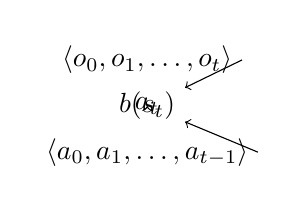
\begin{tikzpicture}
		\matrix [column sep=2em] {
			\node (o) {$\langle o_0, o_1, \dots, o_t \rangle$}; \\
			\&
			\node (s) {$b(s_t)$}; \& \node (an) {$a_t$}; \\
			\node (a) {$\langle a_0, a_1, \dots, a_{t-1} \rangle$}; \\
		};
		\draw [->] (o.east) -- (s);
		\draw [->] (a.east) -- (s);
		\draw [->] (s) -- (an);
	\end{tikzpicture}
\end{center}
where $b(s)$ denotes the belief of $s$, being either a set of states or a
probability distribution. Since each state estimate depends on the whole
sequence of observations, also the next action is implicitly based on the
whole history.

Standard RL algorithms cannot be applied to POMDPs, because the state space is
not observable. Also, since we commonly assume the transition and observation
functions to be unknown, no estimation could be carried out anyway.  There is
a clear difference between MDPs and POMDPs. Still, RL algorithms are
frequently applied to POMDPs. Not surprisingly, they perform very poorly on
these environments. See, for example, the games with worst performances
in~\cite{bib:atari-deepq-nature}. This is a subtle mistake, because
determining whether we're observing the state space is the same as answering
the following question: does the observation space capture the whole dynamics
of the system being observed? Or, more precisely, does an equivalent MDP
$\langle \obsS, A, T_\obsS, R_\obsS, \discount' \rangle$ that produces the
same rewards exist? If both $T_\obsS: \obsS \times A \times \obsS \to \R$ and
$R_\obsS: \obsS \times A \times \obsS \to \R$ exist and produce the same
rewards, the environment can be successfully modelled and solved with an MDP.
Figure~\ref{fig:pomdp-as-mpd} represents this situation.

\begin{figure}
	\centering
	\begin{tikzpicture}[
			hidden node/.style={node, fill=gray},
			hidden arc/.style={->, densely dotted},
			box/.style={rounded corners=5pt, inner sep=1.8ex, draw=#1!50,
				fill=#1!20},
		]
		\matrix [
			column sep={1.6cm,between origins}, row sep={1.3cm,between origins},
		] {
			\node (stm1) [hidden node, label=above:$s_{t-1}$] {}; \& \&
			\node (st) [hidden node, label=above:$s_{t}$] {}; \& \&
			\node (st1) [hidden node, label=above:$s_{t+1}$] {}; \\
			\&
			\node (am1) [node, label=above:$a_{t-1}$] {}; \&
			\node (r) [node, label=left:$r_{t}$] {}; \&
			\node (a) [node, label=above:$a_{t}$] {}; \&
			\node (r1) [node, label=left:$r_{t+1}$] {}; \\
			\node (om1) [node, label=below:$o_{t-1}$] {}; \& \&
			\node (o) [node, label=below:$o_{t}$] {}; \& \&
			\node (o1) [node, label=below:$o_{t+1}$] {}; \\
		};
		\draw [hidden arc, bend left] (stm1) to (om1);
		\draw [hidden arc, bend left] (st) to (o);
		\draw [hidden arc, bend left] (st1) to (o1);
		%
		\draw [hidden arc] (st) -- (r);
		\draw [hidden arc] (st1) -- (r1);
		%
		\draw [hidden arc] (stm1) -- (st);
		\draw [hidden arc] (st) -- (st1);
		\draw [hidden arc] (am1) -- (st);
		\draw [hidden arc] (a) -- (st1);
		%
		\draw [dashed, gray] (st1) -- +(0.8,0);
		\draw [dashed, gray] (stm1) -- +(-0.8,0);
		%
		\draw [->] (o) -- (r);
		\draw [->] (o1) -- (r1);
		%
		\draw [->] (om1) -- (o);
		\draw [->] (o) -- (o1);
		\draw [->] (am1) -- (o);
		\draw [->] (a) -- (o1);
		%
		\draw [dashed, gray] (st1) -- +(0.8,0);
		\draw [dashed, gray] (stm1) -- +(-0.8,0);
		\draw [dashed, gray] (o1) -- +(0.8,0);
		\draw [dashed, gray] (om1) -- +(-0.8,0);
		% boxes
		\begin{pgfonlayer}{below}
			\path coordinate (st-up) at ($(st)+(0,1em)$);
			\node [fit={(stm1) (st1) (st-up)}, box=gray,
				pin=right:{\footnotesize hidden dynamics}
			] {};
			\node [fit={(om1) (o1) ($(a.north)+(0,1ex)$) ($(o.south)+(0,-1ex)$)},
				box=orange, pin=right:{\footnotesize MDP assumption}] {};
		\end{pgfonlayer}
	\end{tikzpicture}
	\caption{The dotted arrows \protect\tikz [baseline=-0.5ex] \protect\draw
	[densely dotted, ->] (0,0) to +(1.5em,0); represent the dependencies in a
	POMDP model. Solid arrows \protect\tikz [baseline=-0.5ex] \protect\draw
	[->] (0,0) to +(1.5em,0); show the MDP model over the same quantities.}
	\label{fig:pomdp-as-mpd}
\end{figure}

\begin{example}
	As we've seen from Example~\vref{ex:board-games}, the game of Chess can
	be modelled with an MDP if we consider as states the vectors of positions of
	all pieces on the board. Let's suppose, instead, the observations available
	are images of the board after each move (if the pieces can be distinguished,
	these could even come from a real play). Each image completely captures the
	state of the game because, for each move of the agent and the opponent,
	we're able to accurately predict image that will follow. This is a
	transition $T_\obsS$ over images. Similarly, a reward function $R_\obsS$ can
	simply return $+1$ or $-1$ for images with checkmates and 0 otherwise. These
	functions can be unknown and don't need to be defined.

	Suppose, instead, that the agent can only observe the left-hand side of the
	board (columns a-d, for example). In this case, each image provides an
	incomplete view over the state of the game. In fact, in order to determine
	the best action we must consider whether there are some attacking pieces on
	the hidden region. In this case, classic RL algorithms would perform poorly,
	because an image it's not sufficient to predict the next image and reward.
\end{example}

\begin{example}
	Let's consider a classic control problem: the swing-up of an inverted
	pendulum. A pendulum can freely rotate by 360° around a hinge. The agent, at
	each discrete time step, can apply torques to this active joint.  The goal
	is to stabilize the pendulum in the upward position, which is the
	configuration of unstable equilibrium. In order to solve this problem with
	Reinforcement Learning, we need to define the spaces $S$ and $A$ of the MDP.
	In this domain, actions are continuous torques. So, assuming a normalized
	range, $A \coloneqq [-1, +1] \subseteq \R$. The angle of the pendulum
	$\theta$ with respect to some fixed reference completely determines the
	position of the masses. Is the reward Markovian with respect to $S =
	\{\theta \in [-\pi, +\pi]\}$? No, because the agent is rewarded when the
	pendulum stops in the upward position. So, the appropriate state space
	consists of both $\theta$ and $\dot\theta$ (or, rather its discrete-time
	approximation).

	Including the momentum in the state space is very common for mechanical
	systems. However, this can be also necessary for games. In fact, just
	looking at a single frame, the agent has no clue about how all the elements
	in the picture are moving.  For example, an optimal policy would take into
	account the direction of an approaching ball in order to hit it.
\end{example}


\subsection{Temporally-extended goals}

The previous section has shown how partial observations may falsify the Markov
assumption on rewards. A second possibility is to have a complete observation
of the state ($\obsS = \stateS$) but a task that is intrinsically
non-Markovian. In this case, each reward is computed from the whole history
of events
\begin{equation}
	r_t = R(\langle s_0, s_1, \dots, s_t \rangle) \qquad \forall t \in \Z
\end{equation}
with $R: \stateS^* \to \R$. The sequence of states $\trace
\coloneqq \langle s_0, s_1, \dots, s_t \rangle$ will be also called
execution \emph{trace}. In general, with the term ``trace'' we indicate any
sequence that is produced during a run. $\trace(i, j)$, with $i \le j$,
denotes a slice of the trace $\trace$ between instants $i$ and $j$;
$\trace(i)$ is the value at time $i$; $\abs{\trace}$ denotes the number of
instants of the sequence; and $\langle \rangle$ is the empty trace.

Why should we define a reward function that is explicitly non-Markovian?
Because, for example, instead of just reaching a desirable state, we might
want our agent to drive the environment through a sequence of states.

\begin{example}
	Let's suppose the agent can control a light bulb through a switch, and we
	want the light to be set on, then off again. This environment is extremely
	simple: its state is completely described by a Boolean variable,
	``lightOn'', which reflects the status of the light. Still, to valuate
	whether the task has been accomplished at time~$t$, it's not sufficient to
	determine whether the light is off in state~$s_t$. Instead, we also need to
	see whether at some previous instant $s_{t'} \prec s_t$ the light was set
	on.
\end{example}

We now define a model that by generalizing MDPs can describe this class of
problems. A \emph{Non-Markovian Reward Decision Process}
(NMRDP)~\cite{bib:nmrdp-logic-first} is a tuple $\langle \stateS, A, T, R,
\discount \rangle$, where $\stateS, A, T, \discount$ are defined as for MDPs,
and $R: \stateS^* \to \R$ is a non-Markovian reward function, which computes
the reward at time $t$ as $r_t = R(\langle s_0, s_1, \dots, s_t \rangle)$.

% TODO: not just sequences
% TODO: temporally-extended goals name

% TODO: Logic that models traces (remove definition of traces)


\section{Reinforcement learning with restraining specifications}
Restraining Bolt method~\cite{bib:bolt}\cite{bib:rb-imitation-l}.

